
\begin{figure}[H]
  {
    \setlength{\tabcolsep}{3.0pt}
    \setlength\cmidrulewidth{\heavyrulewidth} % Make cmidrule = 
    \begin{adjustbox}{width=4cm,center}
      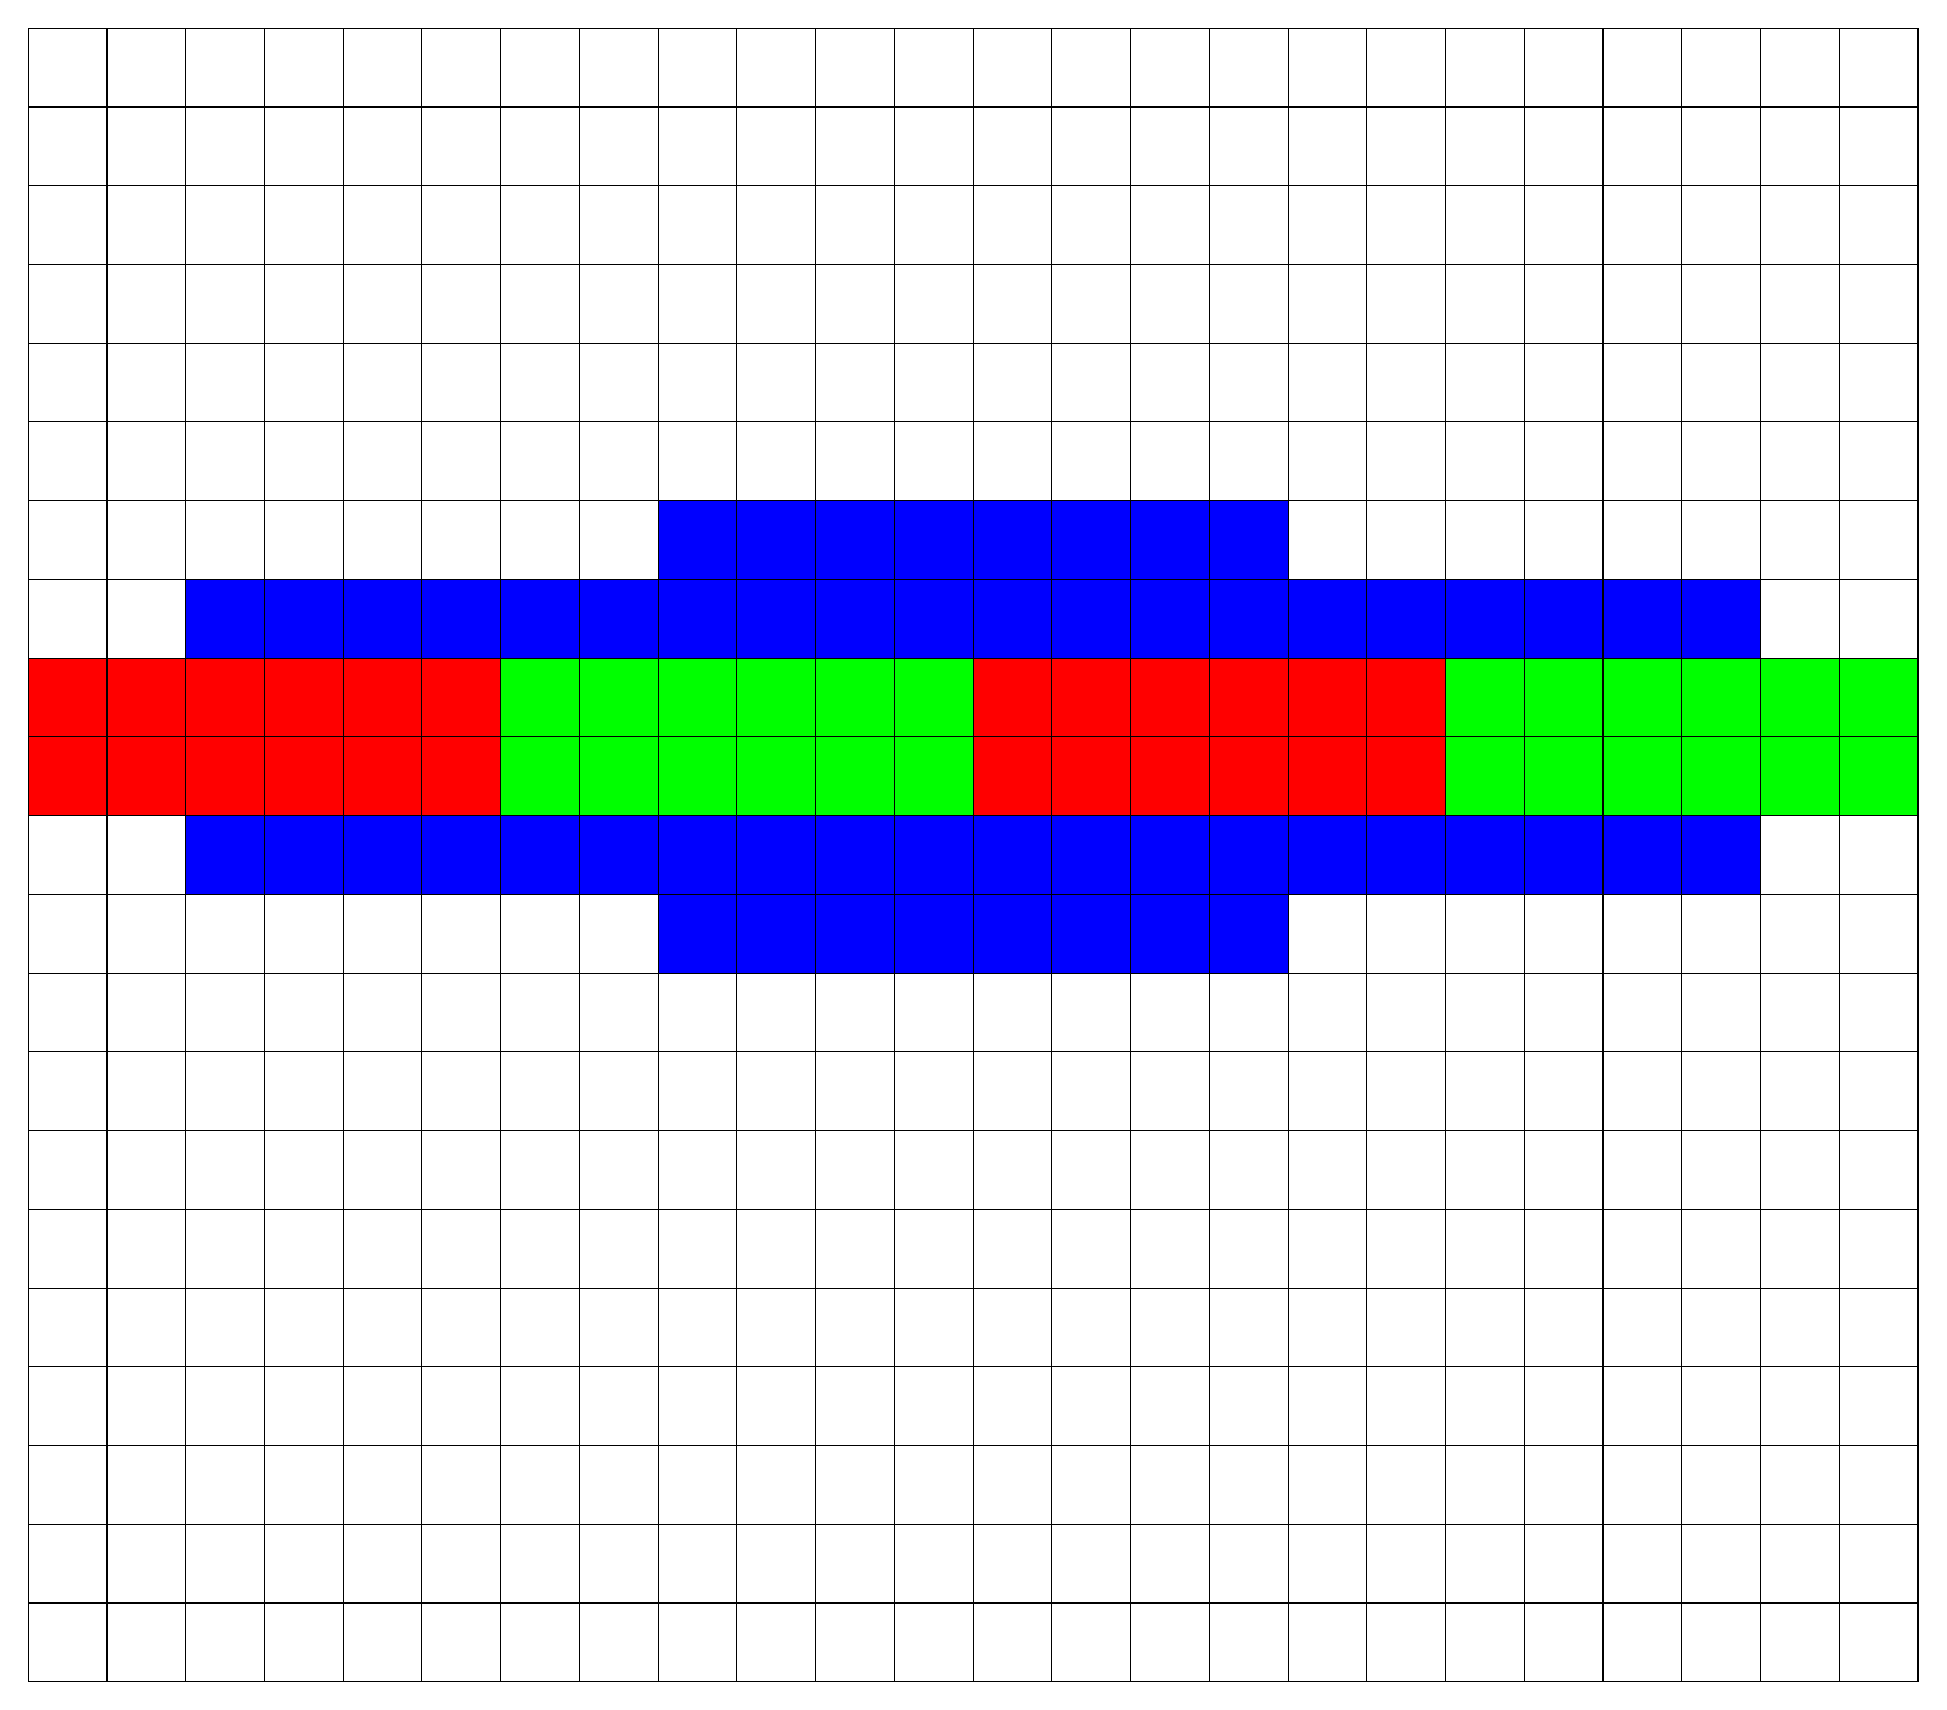
\begin{tikzpicture}

	\fill[blue] (8,14) rectangle ++ (1,1);
	\fill[blue] (9,14) rectangle ++ (1,1);
	\fill[blue] (10,14) rectangle ++ (1,1);
	\fill[blue] (11,14) rectangle ++ (1,1);
	\fill[blue] (12,14) rectangle ++ (1,1);
	\fill[blue] (13,14) rectangle ++ (1,1);
	\fill[blue] (14,14) rectangle ++ (1,1);
	\fill[blue] (15,14) rectangle ++ (1,1);
	\fill[blue] (2,13) rectangle ++ (1,1);
	\fill[blue] (3,13) rectangle ++ (1,1);
	\fill[blue] (4,13) rectangle ++ (1,1);
	\fill[blue] (5,13) rectangle ++ (1,1);
	\fill[blue] (6,13) rectangle ++ (1,1);
	\fill[blue] (7,13) rectangle ++ (1,1);
	\fill[blue] (8,13) rectangle ++ (1,1);
	\fill[blue] (9,13) rectangle ++ (1,1);
	\fill[blue] (10,13) rectangle ++ (1,1);
	\fill[blue] (11,13) rectangle ++ (1,1);
	\fill[blue] (12,13) rectangle ++ (1,1);
	\fill[blue] (13,13) rectangle ++ (1,1);
	\fill[blue] (14,13) rectangle ++ (1,1);
	\fill[blue] (15,13) rectangle ++ (1,1);
	\fill[blue] (16,13) rectangle ++ (1,1);
	\fill[blue] (17,13) rectangle ++ (1,1);
	\fill[blue] (18,13) rectangle ++ (1,1);
	\fill[blue] (19,13) rectangle ++ (1,1);
	\fill[blue] (20,13) rectangle ++ (1,1);
	\fill[blue] (21,13) rectangle ++ (1,1);
	\fill[red] (0,12) rectangle ++ (1,1);
	\fill[red] (1,12) rectangle ++ (1,1);
	\fill[red] (2,12) rectangle ++ (1,1);
	\fill[red] (3,12) rectangle ++ (1,1);
	\fill[red] (4,12) rectangle ++ (1,1);
	\fill[red] (5,12) rectangle ++ (1,1);
	\fill[green] (6,12) rectangle ++ (1,1);
	\fill[green] (7,12) rectangle ++ (1,1);
	\fill[green] (8,12) rectangle ++ (1,1);
	\fill[green] (9,12) rectangle ++ (1,1);
	\fill[green] (10,12) rectangle ++ (1,1);
	\fill[green] (11,12) rectangle ++ (1,1);
	\fill[red] (12,12) rectangle ++ (1,1);
	\fill[red] (13,12) rectangle ++ (1,1);
	\fill[red] (14,12) rectangle ++ (1,1);
	\fill[red] (15,12) rectangle ++ (1,1);
	\fill[red] (16,12) rectangle ++ (1,1);
	\fill[red] (17,12) rectangle ++ (1,1);
	\fill[green] (18,12) rectangle ++ (1,1);
	\fill[green] (19,12) rectangle ++ (1,1);
	\fill[green] (20,12) rectangle ++ (1,1);
	\fill[green] (21,12) rectangle ++ (1,1);
	\fill[green] (22,12) rectangle ++ (1,1);
	\fill[green] (23,12) rectangle ++ (1,1);
	\fill[red] (0,11) rectangle ++ (1,1);
	\fill[red] (1,11) rectangle ++ (1,1);
	\fill[red] (2,11) rectangle ++ (1,1);
	\fill[red] (3,11) rectangle ++ (1,1);
	\fill[red] (4,11) rectangle ++ (1,1);
	\fill[red] (5,11) rectangle ++ (1,1);
	\fill[green] (6,11) rectangle ++ (1,1);
	\fill[green] (7,11) rectangle ++ (1,1);
	\fill[green] (8,11) rectangle ++ (1,1);
	\fill[green] (9,11) rectangle ++ (1,1);
	\fill[green] (10,11) rectangle ++ (1,1);
	\fill[green] (11,11) rectangle ++ (1,1);
	\fill[red] (12,11) rectangle ++ (1,1);
	\fill[red] (13,11) rectangle ++ (1,1);
	\fill[red] (14,11) rectangle ++ (1,1);
	\fill[red] (15,11) rectangle ++ (1,1);
	\fill[red] (16,11) rectangle ++ (1,1);
	\fill[red] (17,11) rectangle ++ (1,1);
	\fill[green] (18,11) rectangle ++ (1,1);
	\fill[green] (19,11) rectangle ++ (1,1);
	\fill[green] (20,11) rectangle ++ (1,1);
	\fill[green] (21,11) rectangle ++ (1,1);
	\fill[green] (22,11) rectangle ++ (1,1);
	\fill[green] (23,11) rectangle ++ (1,1);
	\fill[blue] (2,10) rectangle ++ (1,1);
	\fill[blue] (3,10) rectangle ++ (1,1);
	\fill[blue] (4,10) rectangle ++ (1,1);
	\fill[blue] (5,10) rectangle ++ (1,1);
	\fill[blue] (6,10) rectangle ++ (1,1);
	\fill[blue] (7,10) rectangle ++ (1,1);
	\fill[blue] (8,10) rectangle ++ (1,1);
	\fill[blue] (9,10) rectangle ++ (1,1);
	\fill[blue] (10,10) rectangle ++ (1,1);
	\fill[blue] (11,10) rectangle ++ (1,1);
	\fill[blue] (12,10) rectangle ++ (1,1);
	\fill[blue] (13,10) rectangle ++ (1,1);
	\fill[blue] (14,10) rectangle ++ (1,1);
	\fill[blue] (15,10) rectangle ++ (1,1);
	\fill[blue] (16,10) rectangle ++ (1,1);
	\fill[blue] (17,10) rectangle ++ (1,1);
	\fill[blue] (18,10) rectangle ++ (1,1);
	\fill[blue] (19,10) rectangle ++ (1,1);
	\fill[blue] (20,10) rectangle ++ (1,1);
	\fill[blue] (21,10) rectangle ++ (1,1);
	\fill[blue] (8,9) rectangle ++ (1,1);
	\fill[blue] (9,9) rectangle ++ (1,1);
	\fill[blue] (10,9) rectangle ++ (1,1);
	\fill[blue] (11,9) rectangle ++ (1,1);
	\fill[blue] (12,9) rectangle ++ (1,1);
	\fill[blue] (13,9) rectangle ++ (1,1);
	\fill[blue] (14,9) rectangle ++ (1,1);
	\fill[blue] (15,9) rectangle ++ (1,1);
	\draw (0,0) grid (24,21);

      \end{tikzpicture}
    \end{adjustbox}
  }\caption{FLYING\_SAUCER1}
\end{figure}
